\documentclass[12pt, a4paper,  nobibnotes]{article}

%%%%%%%%%%%%%%%%%
% Configuration %
%%%%%%%%%%%%%%%%%
\usepackage{amsmath}
% If magyar is wanted
\usepackage[T1]{fontenc}
\usepackage[utf8]{inputenc}
\usepackage{fixltx2e}
\usepackage{multirow}
\usepackage{url}
\usepackage{amsfonts}
\usepackage{amsthm}
\usepackage{mathtools}
\usepackage{amssymb}

\usepackage[dvipsnames]{xcolor}
\newcommand{\red}[1]{\textcolor{red}{#1}}

\usepackage{setspace}
\onehalfspacing

% Nice algorithms
\usepackage{algorithm}
\usepackage{algpseudocode}

% Margins 
\usepackage{anysize}
\marginsize{1.64cm}{2.0cm}{1.2cm}{2.4cm} %\left right top bottom

% Multiple languages
\usepackage[english,magyar]{babel}

% using circled symbols
\usepackage{tikz}
\newcommand*\circled[1]{
    \tikz[baseline=(char.base)]{
        \node[shape=circle,draw,inner sep=2pt] (char) {#1}
    }
}

\newcommand{\op}[1]{\hat{#1}}
\newcommand{\ketbra}[2]{|#1\rangle\langle#2|}
\newcommand{\Ketbra}[2]{\left|#1\right\rangle \left\langle#2\right|}

%%%% Some things for fancier look %%%%
\frenchspacing
\setlength{\parskip}{2ex}
\setlength{\headsep}{0,4cm}
\setlength{\headheight}{4pt}

% fej- es lábléc
\usepackage{fancyhdr}
\usepackage{fancyref}
\usepackage{fancyvrb}
\pagestyle{fancy}

\renewcommand{\headrulewidth}{0,05pt}
\renewcommand{\footrulewidth}{0pt}


\fancyhf{}
\fancyhead[RE]{{ \nouppercase{\leftmark}} }
\fancyhead[LO]{{ \nouppercase{\leftmark}} }
\cfoot{--~\thepage~--}
%%%%%%%%%

% For quantum circuits.
\usetikzlibrary{quantikz}

\usetikzlibrary{fadings}
\usetikzlibrary{patterns}
\usetikzlibrary{shadows.blur}
\usetikzlibrary{shapes}

% Here you can configure the layout
\usepackage{geometry}
\geometry{top=1cm, bottom=1cm, left=1.25cm,right=1.25cm, includehead, includefoot}
\setlength{\columnsep}{7mm} % Column separation width

\usepackage{graphicx}

%\usepackage{gensymb}
\usepackage{float}

% For bra-ket notation
\usepackage{braket}

% To have a good appendix
\usepackage[toc,page]{appendix}

\usepackage{abstract}
\renewcommand{\abstractnamefont}{\normalfont\bfseries}
\renewcommand{\abstracttextfont}{\normalfont\small\itshape}
\usepackage{lipsum}

%%%%%%%%%%%%%%%%%%%
% Custom commands %
%%%%%%%%%%%%%%%%%%%
\newcommand{\bb}[1]{\mathbf{#1}}
\newcommand{\dd}{\mathrm{d}}
\newcommand{\Tr}[1]{\mathrm{Tr}\left[#1\right]}
\newcommand{\Sp}[1]{\mathrm{Sp}\left[{#1}\right]}

\newtheorem*{theorem*}{Theorem}
\newtheorem*{definition*}{Definition}
\newtheorem*{example*}{Example}
\newtheorem*{problem*}{Problem}
\newtheorem*{remark*}{Remark}
\newtheorem*{statement*}{Statement}

\newtheorem{theorem}{Theorem}
\newtheorem{definition}{Definition}
\newtheorem{example}{Example}
\newtheorem{problem}{Problem}
\newtheorem{remark}{Remark}
\newtheorem{statement}{Statement}

\usepackage[square,numbers]{natbib}
\bibliographystyle{unsrtnat} %{abbrvnat}

%% COMMENTS
\newcommand{\nd}[1]{\textcolor{Aquamarine}{\textbf{[Dani: #1]}}}

% Hyperref should be generally the last package to load
% Any configuration that should be done before the end of the preamble:

\usepackage{hyperref}
\hypersetup{colorlinks=true, urlcolor=blue, linkcolor=blue, citecolor=blue}

%%%%%%%%%%%%%%%%%%%%%%%%%%%%%%%%%%%%%%%%%%%%%%%%%%%%%%%%%%%%%
%                    BEGIN    DOCUMENT                      % 
%%%%%%%%%%%%%%%%%%%%%%%%%%%%%%%%%%%%%%%%%%%%%%%%%%%%%%%%%%%%%

\begin{document}
\selectlanguage{english}
\begin{center}
\vspace*{5.0cm}
\LARGE{Experimenting with machine learning algorithms on quantum computers}\\
\vspace{2.0cm}
\large{Nagy Dániel$^1$}\\
\vspace{2.0cm}
\large{
    $^1$Institute for Physics, Eötvös Loránd University, H-1117, Pázmány Péter sétány 1/A. Budapest, Hungary\\%
    \vspace{5.0cm}
    Created on December 1, 2019\\
    \vspace{1.0cm}
    Last update: \today
}
\end{center}
\thispagestyle{empty} %% No fancy
\newpage

\begin{center}
    \textbf{Abstract}\\
    \par A modern számítástechnika jelentős eredményei közé tartozik a gépi
    tanulás és mesterséges intelligancia alapvető algoritmusainak kifejlesztése és ezek 
    hasznosságának tesztelése különböző feladatokon. Ugyanakkor az elmúlt években a 
    kvantumszámítás is jelentős fejlődésen ment keresztül, olyannyira, hogy 2019-ben a Google kísérleti
    csapatának sikerült demonstrálnia a kvantumfölényt. A munka során megvizsgáljuk a két terület átfedéséből 
    származó lehetőségeket: klasszikus adatok kvantumos feldolgozását illetve a klasszikus
    gépi tanulás segítségével történő kvantumos hibajavítást.
\end{center}
\thispagestyle{empty} %% No fancy
\newpage

\selectlanguage{magyar}
\begin{center}
\vspace*{5.0cm}
\LARGE{Gépi tanulási algoritmusok vizsgálata kvantumszámítógépeken}\\
\vspace{2.0cm}
\large{Nagy Dániel$^1$}\\
\vspace{2.0cm}
\large{
    $^1$Eötvös Loránd Tudományegyetem, Fizika Intézet, H-1117, Pázmány Péter sétány 1/A. Budapest, Magyarország\\%
    \vspace{5.0cm}
    Elkezdve: December 1, 2019\\
    \vspace{1.0cm}
    Utolsó frissítés: \today
}
\end{center}
\thispagestyle{empty} %% No fancy
\newpage


\begin{center}
    \textbf{Kivonat}\\
    \par A modern számítástechnika jelentős eredményei közé tartozik a gépi
    tanulás és mesterséges intelligancia alapvető algoritmusainak kifejlesztése és ezek 
    hasznosságának tesztelése különböző feladatokon. Ugyanakkor az elmúlt években a 
    kvantumszámítás is jelentős fejlődésen ment keresztül, olyannyira, hogy 2019-ben a Google kísérleti
    csapatának sikerült demonstrálnia a kvantumfölényt. A munka során megvizsgáljuk a két terület átfedéséből 
    származó lehetőségeket: klasszikus adatok kvantumos feldolgozását illetve a klasszikus
    gépi tanulás segítségével történő kvantumos hibajavítást.
\end{center}
\thispagestyle{empty} %% No fancy
\newpage

\selectlanguage{english}
% Add a link target to the TOC itself
\addtocontents{toc}{\protect\hypertarget{toc}{}}
\thispagestyle{empty}
\tableofcontents
\newpage

\thispagestyle{empty}
\listoffigures
\newpage

\section{Introduction}
Quantum computing is probably the most promising emerging technology with many possible applications across
all domains of science and business. The idea of quantum computing was first proposed by Richard P. Feynman
as a method to simulate quantum mechanics. Since the size of the Hilbert-space grows exponentially with
the complexity of the quantum system, and thus the calculations become intractable on any classical
computer, Feynmans idea was to simulate quantum physics on devices that behave themselves according to 
the rules of quantum physics.
\par
Soon after Feynmans proposal, scientists became to establish the theoretical background of quantum
information and quantum computing. Some of the quantum algorithms are proven to have an 
advantage over any known classical algorithm. One of the first such quantum algorithm is 
the Deutsch-Jozsa algorithm \cite{DeutschJozsa1992}, which decides if a binary function $f$ 
is balanced or constant. Probably the most notable quantum algorithm was proposed by Peter W. Shor 
in 1994, which is a polynomial-time quantum algorithm for factoring large integers \cite{Shor1994}.
This is the first quantum algorithm with a real-life application, because most of the public-key
cryptosystems could be broken with an efficient algorithm for integer factoring. 
Another important quantum algorithm is the Grover's algorithm proposed by Lov K. Grover in 1996 for
searching an unordered database \cite{Grover1996}. While the best known classical algorithm 
for searching unordered databases runs in $O(N)$ time, Grover's algorithm solves this problem
with $O(\sqrt N)$ oracle queries. Beyond quantum algorithms, many quantum-inspired algorithms were 
discovered \cite{Tang2019,Ding2019QuantumInspiredSVM,ArrazolaQuantumInspired2019}.

\section{Quantum Computing with continuous variables}
\nd{cite: Xanadu paper, Photonic Supremacy paper, PsiQuantum Fusion-Based QC}
Continuous variable (CV) systems have infinite degrees of freedom, and therefore the corresponding Hilbert-space is of infinite dimensions. 
Such systems can be modeled by $M$ harmonic oscillators, which are usually called \textit{modes}. 
% each having a Hilbert-space $\mathcal H_k$. 
With $H_k$ denoting the Hilbert-space of the $k$th mode, the Hilbert-space of the full CV system is their direct sum:
\begin{equation}
    \mathcal H = \bigoplus\limits_{k=1}^M\mathcal H_k.
\end{equation}
The Hamiltonian of mode $j$ can be described by introducing bosonic creation and annihilation operators $a_j^\dagger$ and $a_j$, obeying the following canonical commutation relations:
\begin{align}
    \left[\op a_j, \op a_k^\dagger \right] = \delta_{jk}, & \left[\op a_j^\dagger, \op a_k^\dagger\right] = \left[\op a_j, \op a_k\right] = 0.
\end{align}
The effect of the creation and annihilation operators on the Fock space can be described by the 
following identities:
\begin{align}
    \begin{split}
    &\op a_k^{\dagger} \ket{n_1, \dots, n_k, \dots} = \sqrt{1+n_k}\ket{n_1, \dots, n_k + 1, \dots} \\
    &\op a_k \ket{n_1, \dots, n_k, \dots} = \sqrt{n_k} \ket{n_1, \dots, n_k - 1, \dots} \\
    \end{split}
\end{align}
We also introduce the number operator $\op n_j=\op a_j^\dagger \op a_k$:
\begin{align}
 &\op a_k^\dagger \op a_k |n_1, ..., n_k, ... \rangle = \op n_k |n_1, ..., n_k, ... \rangle = n_k |n_1, ..., n_k, ... \rangle
\end{align}
Each of the single-mode Hilbert-space $\mathcal H_k$ is an infinite-dimensional Fock-space spanned by the eigenvectors 
of the number operator $\op n_k = \op a_k^\dagger \op a_k$ labeled $\{\ket{n}\}_k$.
It is often useful to introduce the canonical position operators $X_j$ and momentum operators $P_j$ which are related to the creation and annihilation operators
by the following transformations:
\begin{align}
  \op X_k &= \frac{\op a_k+\op a_k^\dagger}{\sqrt{2}}  & \op a_k &= \frac{\op X_k + i\op P_k}{\sqrt{2}}  \\ 
  \op P_k &= \frac{\op a_k-\op a_k^\dagger}{i\sqrt{2}} & \op a_k^\dagger &= \frac{\op X_k - i\op P_k}{\sqrt{2}}
   \label{eq:jwtransform}
\end{align}
Operators $\op X_k$ and $\op P_k$ are called quadrature operators. Following the notation often used in literature, we group these operators into a vector 
\begin{equation}
    \mathbf R^\top = (\op X_1, \op P_1, \op X_2, \op P_2, ..., \op X_k, \op P_k, ..., \op X_M, \op P_M)
    \label{eq:xidef}
\end{equation}
We can calculate the commutators $\left[\mathbf R_k,\mathbf R_l\right]$ by introducing a symplectic form $\pmb\Omega$ as
\begin{equation}
    \pmb\Omega = \bigoplus\limits_{j=1}^{M}\pmb\omega,~\pmb\omega = 
    \begin{pmatrix}
    0 & 1 \\
    -1 & 0
    \end{pmatrix}.
\end{equation}
Using this notation, we can write
\begin{equation}
    \left[\mathbf R_k,\mathbf R_l\right] = i\pmb\Omega_{kl}
\end{equation}

Apart from the Fock-basis, there is another useful alternative basis, the basis of \textit{coherent states},
which are eigenstates of the annihillation operator $\op a_k$:
\begin{equation}
    \op a_k \ket{\alpha}_k = \alpha\ket{\alpha}_k,
\end{equation}
with $\alpha\in\mathbb C$. From definition this, we can derive that the Fock-basis expansion of 
the coherent state $\ket\alpha_k$ is
\begin{equation}
    \ket\alpha_k = e^{-\frac{1}{2}|\alpha|^2}\sum\limits_{n=1}^\infty \frac{\alpha^n}{\sqrt{n!}}\ket n_k.
\end{equation}
The derivation of the above formula is explained in detail in appendix \ref{appendix:coherent}. By introducing 
the single-mode Weyl-displacement operator 
\begin{equation}
    \op D_k(\alpha) = e^{\alpha\op a^\dagger_k - \alpha^*\op a_k},
\end{equation}
we can create coherent states from the vacuum state: $\ket\alpha_k = \op D_k(\alpha)\ket 0_k$. Of 
course, we can define multimode coherent states 
\begin{equation}
    \ket{\alpha_1}_1 \otimes \ket{\alpha_2}_2 \otimes \cdots \otimes \ket{\alpha_N}_N \equiv \ket{\pmb\xi} = \op D(\pmb\xi) \ket 0,
\end{equation}
where $\op D(\pmb\xi)$ is the multi-mode Weyl-displacement operator defined as
\begin{equation}
    \op D(\pmb\xi) = e^{i\mathbf R^\top\pmb\Omega\pmb\xi}, ~ \pmb\xi \in \mathbb R^{2N}.
\end{equation}
For a single mode, 
\begin{equation}
    \op D_k(\pmb\xi) = \op D_k\left(\begin{matrix}
        \xi_1 \\ \xi_2
    \end{matrix}\right)
    = e^{i(\xi_2 \op X_k - \xi_1 \op P_k)},\,\textrm{if we set}\,\left(\begin{matrix}
        \xi_1 \\ \xi_2
    \end{matrix}\right) = \frac{1}{\sqrt 2}\left(\begin{matrix}
        \textrm{Re}(\alpha_k) \\ \textrm{Im}(\alpha_k)
    \end{matrix}\right)
\end{equation}

\nd{Write about phase-space, quasiprobability}
\nd{Write about different quantum gates.}
\nd{Write about homodyne measurements, heterodyne measurements and photon number-resolving measurements}


\section{Machine learning}

Machine learning is simply said, a new paradigm in software development. Traditional software have
a predefined behaviour, which does not change over time. In contrast, machine learning models
are iteratively "trained" i.e. updated to achieve better performance by the use of data. These algorithms
are designed to learn patterns from the data available and update themselves with new experience.
Although, there are a lot of machine learning algorithms, they usually fit into one of the following three 
main classes:
\begin{itemize}
    \item \textbf{Supervised Learning}. Supervised Learning (SL) algorithms need labeled data, and
    based on the input-output pairs previously seen by the algorithm, it learns to produce
    correct outputs for previously unseen inputs. A very basic example of supervised learning 
    is the linear regression or support vector machines \nd{ref?} for classification, but there are a lot of complex models like CNNs for image classification
    \nd{ref?}, which are trained in a supervised manner.  
    \item \textbf{Unsupervised Learning}. Unsupervised Learning (UL) does not require labeled data, instead
    of that, it is trying to learn from a lot of unlabeled data points. These algorithms include a bunch
    of clustering methods, like k-means \nd{ref?}, or mixture models \nd{ref?}. Another example of unsupervised
    learning is latent variables or distributions for feature extraction or data denoising. A great example 
    of latent distribution learning are Variational Autencoders \cite{VAEPaper} which have bean adobted 
    for a variety of tasks.
    \item \textbf{Reinforcement Learning}. Reinforcement Learning (RL) is very different from the previously
    mentioned two classes of machine learning method. In RL the goal is not to learn from a given set of 
    data, but rather to solve a specific task in an environment. In RL, an \textit{agent} learns to 
    perform a task by observing the state (or some subspace of the state) of the surrounding environment,
    and executing actions in order to maximize an objective. RL is inspired by the process of learning from 
    mistakes or rewards. The environment in RL can be any type of physical simulation, or even a computer game.
    Examples for RL algorithms include Deep Q-networks \cite{RLAtariDQN} or AlphaGo \cite{Silver2016AlphaGo}
\end{itemize}

\subsection{Supervised Classification and Regression}
The two most common SL tasks are \textbf{classification} and \textbf{regression}. Both classification
and regression can be performed with traditional algorithms or deep neural networks. In this
chapter we present the basic ideas and formalisms of classification and regression which will be 
useful in the following chapters.

In supervised learning the data points consist of pairs $(\mathbf x_i, \mathbf y_i)$, where
$\mathbf x_i$ are called feature vectors and $\mathbf y_i$ are called labels. Both the feature vectors
and the labels are real-valued vectors of any dimension. Feature vectors can be pre-processed to 
achieve better performance. A dataset is usually split into two or three parts. The first part is usually the largest,
which is called the training set, and this is used to train the model. The second dataset 
is called testing or evaluation set and is used to evaluate how the model performs when it is 
fed with previously unseen data. There might be an additional set called the validation set,
which is used to verify the model's performance after training is finished. While the testing 
set is used to monitor the learning process during training, the validation set is used only after
the full training process is finished.

\subsubsection{Classification}
In classification, each point $\mathbf x$ is in one of $K$ predefined categories. That is, 
the labels are integers less or equal to $K$: $y_i \in \{1, ..., K\}$. The goal of a classifier 
is to learn the connection between $\mathbf x_i$ and $y_i$, in other words, to learn, how to 
put each vector $\mathbf x_i$ into the right category. The performance of a classifier is usually measured
with categorical accuracy i.e. what percentage of the predicted labels are in the right category.
Apart from accuracy, it is often useful to introduce the categorical cross-entropy. In general, the 
crossentropy of two probability distributions $p$ and $q$ is defined as 
\begin{equation}
    H(p,q) = -\int p(x)\log q(x)\dd x
\end{equation}
\nd{Explain the intuition behind entropy, cross-entropy etc.}
To transform this general formula of cross-entropy to the case of classification, we need to introduce
one-hot encoding. One-hot encoding maps integer labels to binary vectors in a way that vector 
corresponding to the label $j$ will contain $1$ at the $j$th position and $0$ everywhere else. The
length of the resulting vectors is $K$. For example the one-hot encoding of labels $1$ and $3$ in case of 
three categories would look like
\begin{align}
    \textrm{OneHot}(1,3) = \begin{bmatrix}
        1\\0\\0
    \end{bmatrix}
    &&\textrm{OneHot}(3,3) = \begin{bmatrix}
        0\\0\\1
    \end{bmatrix}
\end{align}

In machine learning, especially in deep learning one-hot encoding of categorical features or labels
is proven to be very useful. Now, with one-hot encoded labels, we can easily define the categorical
crossentropy:
\begin{equation}
    \textrm{CrossEntropy}(\mathbf y^{\textrm{pred}}, \mathbf y^{\textrm{true}})
    = -\sum\limits_{i=1}^K y_i^{\textrm{true}} \log y_i^{\textrm{pred}} 
\end{equation}
The crossentropy essentially measures how the predicted distribution of labels differs from the 
true distribution, hence it is widely used in machine learning.
Applications of classification include image recognition, image segmentation, speech and voice recognition,
fraud detection and a lot more. 
\subsubsection{Regression}
Regression models are usually used 
for forecasting and prediction, or simply to uncover the relationships between two or more features.
Opposed to classification, in regression, the output of the model is not restricted to 
a discrete set of predefined classes, instead the set of possible outputs is a 
bounded or unbounded subset of $\mathbb R^d$. Therefore, classification is a
special case of regression where the set of possible values of the outcomes is 
a finite set of integers.
Apart from this difference, the purpose of regression is the same: to find a connection 
between the features $\mathbf x$ and labels $\mathbf y$. 
The elements of feature vectors $x_i$ are usually called independent variables or predictors, 
while the elements of the label vectors $y_i$ are called dependent variables.
Formally the regression model is a function approximator, which is itself a function that can be 
parametrized by a set of real parameters $\pmb \theta\in \mathbb R^m$. Given a set of observations 
$\{(\mathbf x_1, y_1), (\mathbf x_2, y_2), ... (\mathbf x_N, y_N)\}$ a function approximator $f(\cdot;\pmb\theta)$,
we can write
\begin{equation}
    y_i = f(\mathbf x_i; \pmb\theta) + \epsilon_i,
\end{equation}
Where $\epsilon_i$ denotes a random statistical noise, usually assumed to follow Gaussian distribution.
The goal is to find an optimal set of parameters $\pmb\theta^*$ which minimizes the mean squared 
error:
\begin{equation}
    \pmb\theta^* = \underset{\pmb\theta}{\arg\min}\sum\limits_{k=1}^N(y_k - f(\mathbf x_k;\pmb\theta))^2
\end{equation}
The mean squared error is itself a good measure of the performance of the regression model and
is often used in machine learning and deep learning. Another scalar value for 
getting some information about the 
goodness of fit is the coefficient of determination or often called $R^2$-score.
The $R^2$-score is a real value usually falling between zero and one (the latter meaning 
perfect fit), although sometimes it can be negative.
The $R^2$-score measures the proportion of variance in the predictions that can be 
explained by the data.
To calculate the $R^2$-score, we first introduce the total sum of squares
\begin{equation}
    SS_{\textrm{tot}} = \sum\limits_{i}(y^{\textrm{true}}_i-\langle y^{\textrm{true}} \rangle)^2,
\end{equation}
where $\langle y^{\textrm{true}} \rangle =\frac{1}{N} \sum\limits_{k}y_k^{\textrm{true}}$ is the
mean of the dependent variable in the dataset. Then we calculate the sum of squared residuals,
or sum of squared errors:
\begin{equation}
    SS_{\textrm{res}} = \sum\limits_{i}(y^{\textrm{true}}_i-y^{\textrm{pred}}_i)^2.
\end{equation}
With these two quantities, we can now define the $R^2$-score as follows:
\begin{equation}
    R^2 = 1-\frac{SS_{\textrm{res}}}{SS_{\textrm{tot}}}.
\end{equation}

\subsection{Deep Neural Networks and backpropagation}
Probably the most successful machine learning models are deep neural networks, which enjoy a great 
popularity in the recent years because of their flexibility and expressive power \cite{LeCun2015DeepLearning}.
The training of deep neural networks for various machine learning task
became possible after the proposal of back-propagation algorithm in 1986 by 
Geoffrey Hinton et. al. \cite{BackpropPaper}.


\begin{figure}[H]
    \centering
    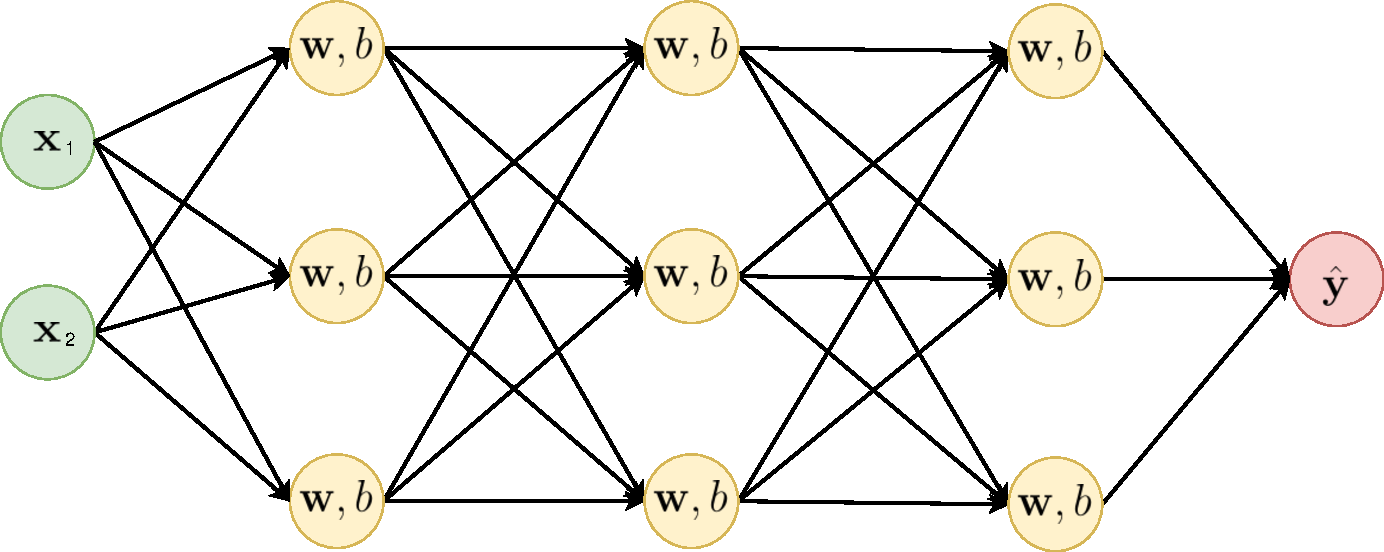
\includegraphics[width=0.7\textwidth]{figures/MLP.pdf}
\end{figure}
\section{Quantum Machine Learning}
QSVM paper = \cite{QSVMPaper}
HHL paper = \cite{HHLPaper}
Feature Hilbert Spaces = \cite{FeatureHilbertSpaces}
Cv-Qnns -LLoyd = \cite{CVQNNLLoyd}
\nd{related papers: quantum svm, Kernel methods, HHL algorithm for matrix inversion, quantum-inspired classical algos\\
motivation: summary from Lloyd paper, regression, classification, hybrid traning, encoding, inference\\
General structure: encoding, rotations and beamsplitter = interferometer, squeezing, interferometer, displacement, all = affine transformation + at the end non-linear, e.g., cubic phase operation (numeric instability switch to Kerr gates --> write at the performance test)  \\
Loss functions: regression, classification\\
Regularization: keep trace close to zero, non-Gaussian\\
}
\subsection{Parametric quantum circuits}
\subsection{Variational Quantum Eigensolver}
\label{sec:vqe}
Variational Quantum Eigensolvers \cite{Peruzzo2014} are hybrid quantum-classical algorithms designed to find the lowest energy eigenvalue of some Hamiltonian $H$. VQEs are one of the most studied quantum algorithms because of their expected use cases in quantum chemistry and
materials science \cite{Wei2020-QCHEM,VQE-HARTREE-FOCK,Kandala2017-VQE-QCHEM,PhysRevX-VQE-QCHEM}.
The basic idea behind the variational quantum eigensolver is as follows. 
First we fix the structure of a parametric quantum circuit called the ansatz, defined by a 
unitary $U(\pmb\theta)$, where $\pmb\theta\in\mathbb{R}^m$ are real parameters. 
Then we start by some initial state $\ket{\psi_0}$, which is usually $\ket 0^{\otimes M}$ 
in the qubit setting. For the continuous variable setting, the initial state can be the vacuum state,
a displaced state, a squeezed state, or a photon number eigenstate.
After preparing the circuit, we evaluate the expectation value of the Hamiltonian
which is eventually the cost, or loss:
\begin{equation}
    \mathcal L(\pmb\theta) = \langle H \rangle = \bra{\psi_0}U^{\dagger}(\pmb\theta)HU(\pmb\theta)\ket{\psi_0}
\end{equation}
The goal is to minimize the loss $\mathcal L$ by iteratively updating the parameters $\pmb\theta$ with some update rule. This update rule can be any gradient-free \cite{Zhu2019} or gradient-based method \nd{idezet}. To use gradient descent optimization in the VQE setting, we need to evaluate the gradient
$\nabla_{\pmb\theta}\mathcal L$, which can be challenging, and is described in details in chapter \ref{sec:qgrad}. Algorithm \ref{algo:vqe} describes 
the variational quantum eigensolver with a general gradient-based learning method. Notice that we wrote $\alpha_j^{(t)}$ for the learning rate, since in most modern optimizers like Adam \cite{Kingma2015AdamAM}, each parameter has its own learning rate and it may depend on the number of iterations already done.
\begin{algorithm}[H]
    \caption{VQE}
    \begin{algorithmic}[1]
    \Procedure {VQE}{$H,K,T,\alpha$}
        \ForAll {$t \in \{1,...,T\}$}
            \State Prepare the ansatz $U(\pmb\theta)$
            \State Estimate the loss $\mathcal L = \bra{\psi_0}U^{\dagger}(\pmb\theta)HU(\pmb\theta)\ket{\psi_0}$ by averaging $K$ shots
            \ForAll{$\theta_j \in \pmb\theta$}
                \State Calculate the quantum gradient $\partial_{\theta_j}\mathcal L$
                \State Update the parameter $\theta_j \leftarrow \theta_j - \alpha_j^{(t)}\partial_{\theta_j}\mathcal L$
            \EndFor
        \EndFor
    \EndProcedure
    \end{algorithmic}
    \label{algo:vqe}
\end{algorithm}

\subsection{Calculating the gradients of the parameters}
\label{sec:qgrad}
In this section, we introduce the theory of calculating quantum gradients in the continuous variable setting. 
We follow the notation of Shuld et. al. \cite{AnalyticGradientsSchuld}. A variational quantum circuit is 
defined by a unitary $U(\pmb\theta),\, \pmb\theta\in\mathbb{R}^m$, an initial state $\ket{\psi_0}$ and a measurment 
operator $B$. We can understand a variational citcuit as $f:\mathbb{R}^m \rightarrow \mathbb{R}$, \nd{The Schuld paper writes $f:\mathbb{R}^m \rightarrow \mathbb{R}^{\red n}$, maybe a typo???} 
which maps the circuit parameters to the expectation value of operator $B$:
\begin{equation}
    f(\pmb\theta) = \bra{\psi_0}U^{\dagger}(\pmb\theta) B U(\pmb\theta)\ket{\psi_0}   
\end{equation}
In gradient-based optimizations, we need the gradient $\nabla_{\pmb\theta} f$, and this eventually means calculating the partial derivatives
$\partial_{\mu}f,\,\mu\in\pmb\theta$. In the continuous variable setting, observables are usually polynomials of the quadrature operators $X_j$ and $P_j$.



\section{Results}
\subsection{Regression}

\begin{equation}
    \mathcal L = \frac{1}{|\mathcal B|}\sum\limits_{(x,y)\in\mathcal B}({y - \bra{\psi_0}\op U^{\dagger}(x;\pmb\theta)\op X_2 \op U(x;\pmb\theta)\ket{\psi_0}})^2 + \frac{\lambda}{|\mathcal B|}\sum||W^{\textrm{active}}||^2 
\end{equation}

\begin{figure}[H]
    \centering
    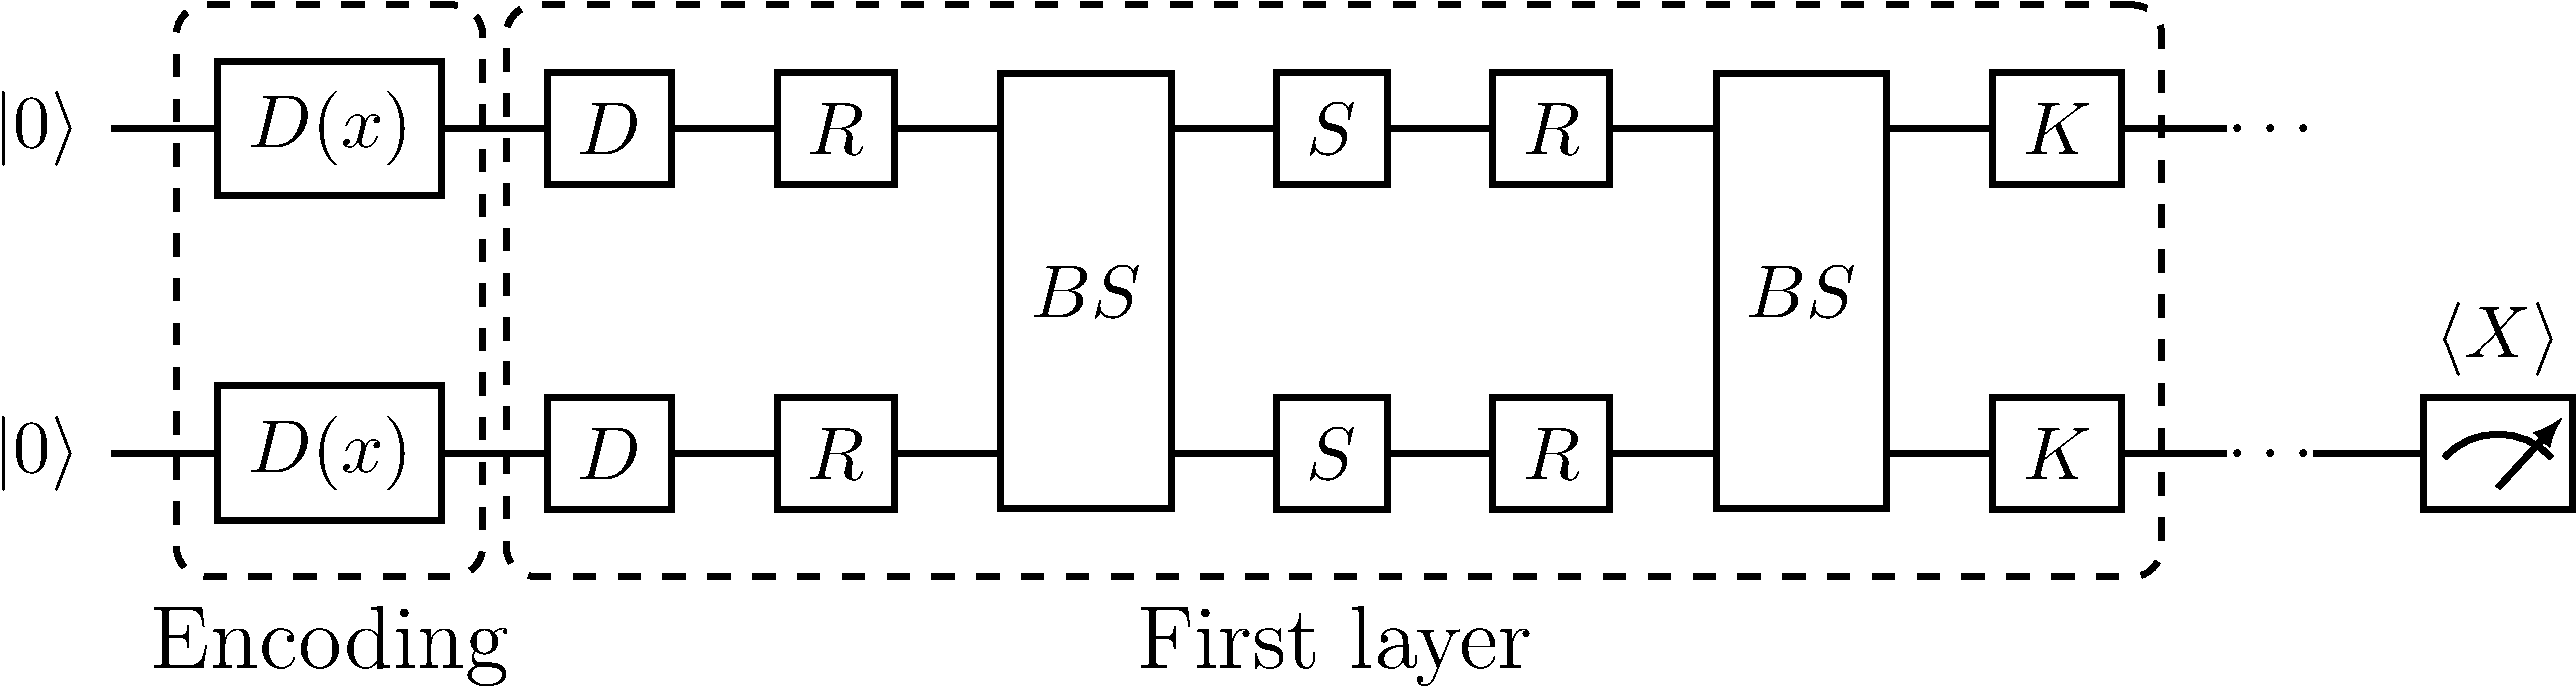
\includegraphics[width=0.75\textwidth]{figures/BasicTwoModeRegressor-circuit.pdf}
    \caption{}
    \label{fig:single_layer_regression}
\end{figure}

\subsection{Classification}
\begin{figure}[H]
    \centering
    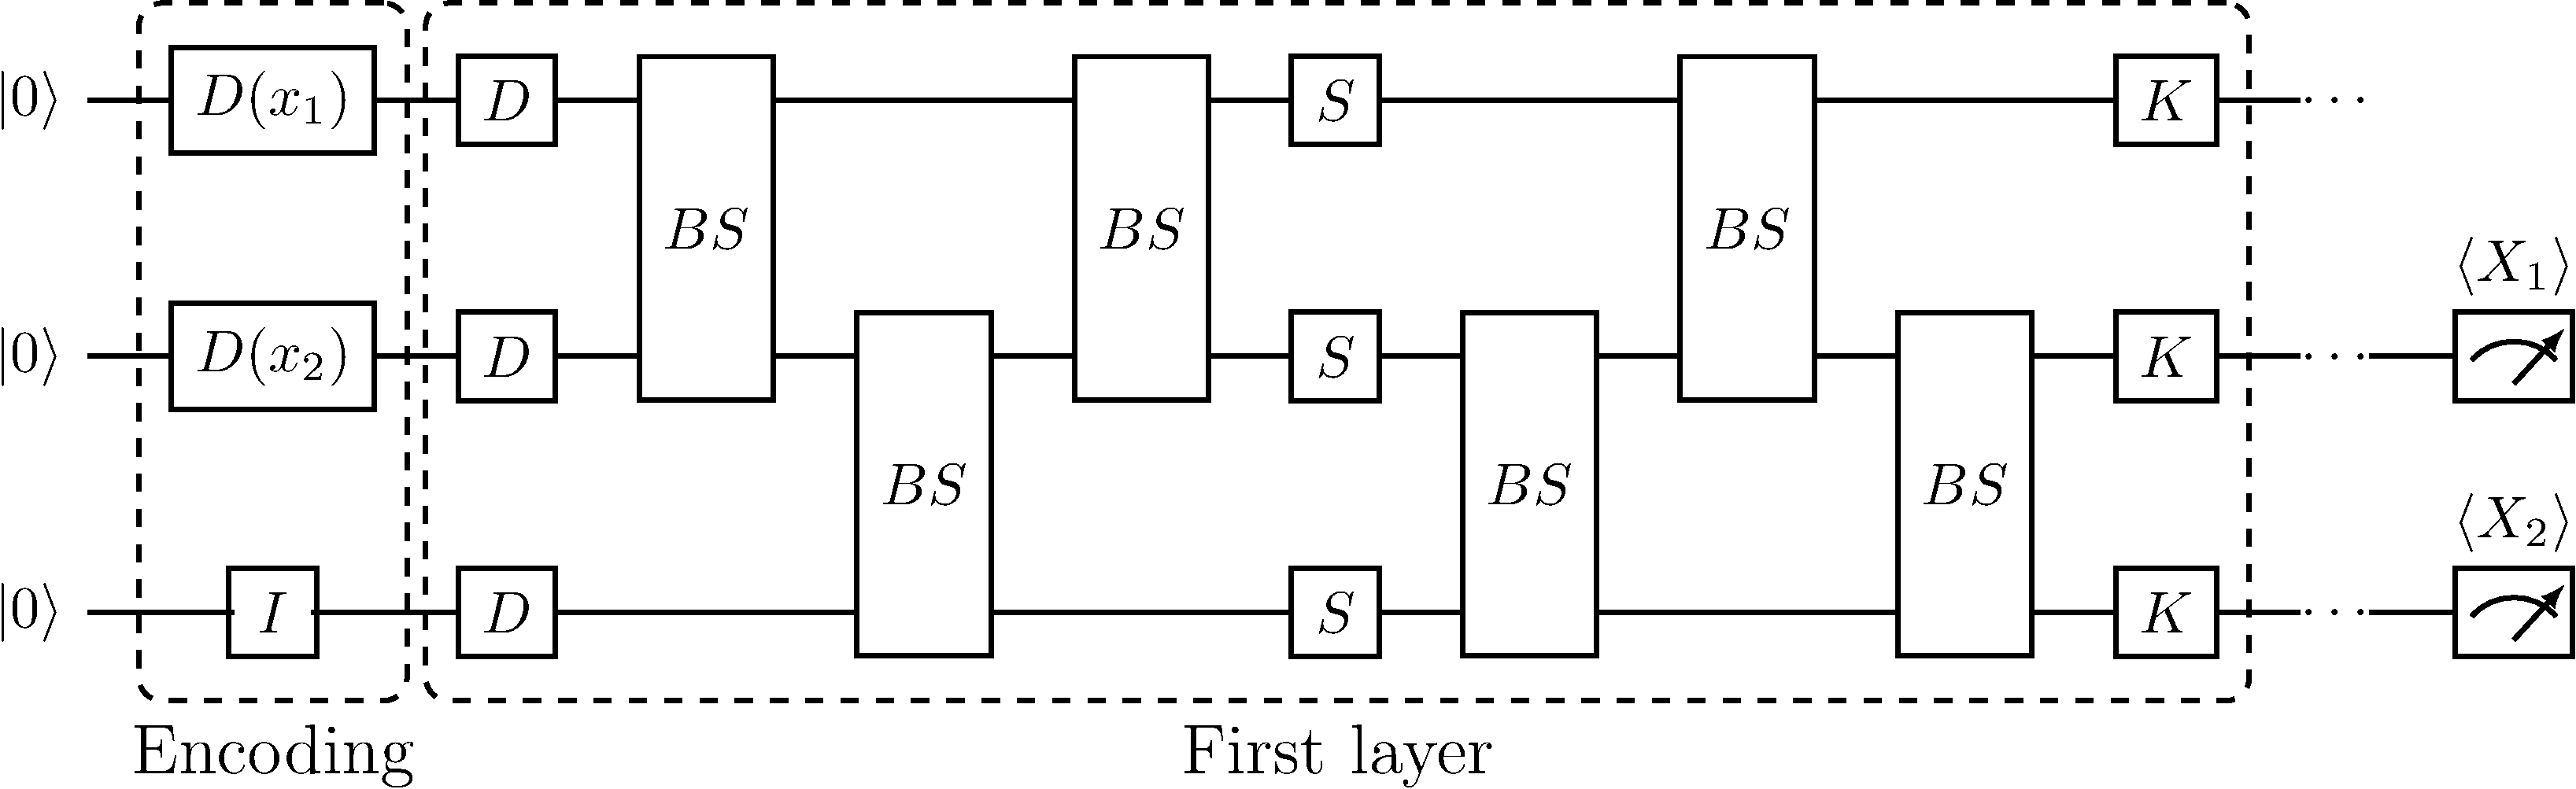
\includegraphics[width=0.75\textwidth]{figures/Classifier-Circles-Ansatz.pdf}
    \caption{}
    \label{fig:single_layer_classification}
\end{figure}


\newcommand{\thisfigurewidth}{0.31}
\begin{figure}[H]
    \centering
    \begin{tabular}{ccc}
      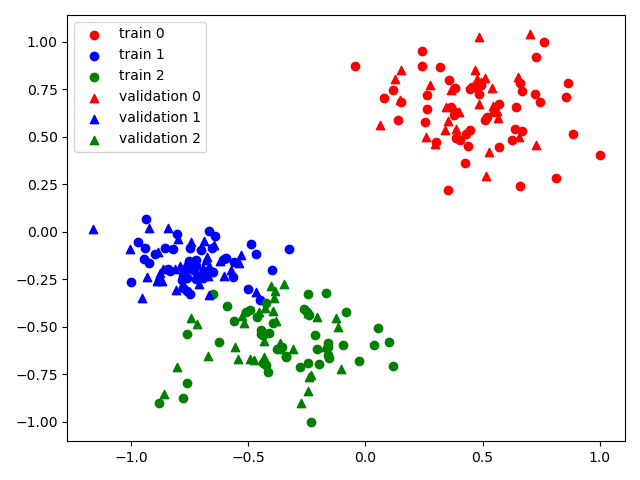
\includegraphics[width=\thisfigurewidth\textwidth]{figures/fig_dataset_blobs.png} & 
      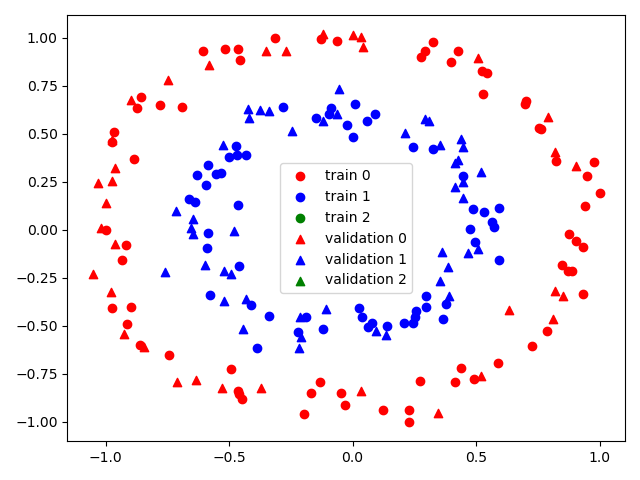
\includegraphics[width=\thisfigurewidth\textwidth]{figures/fig_dataset_circles.png} &
      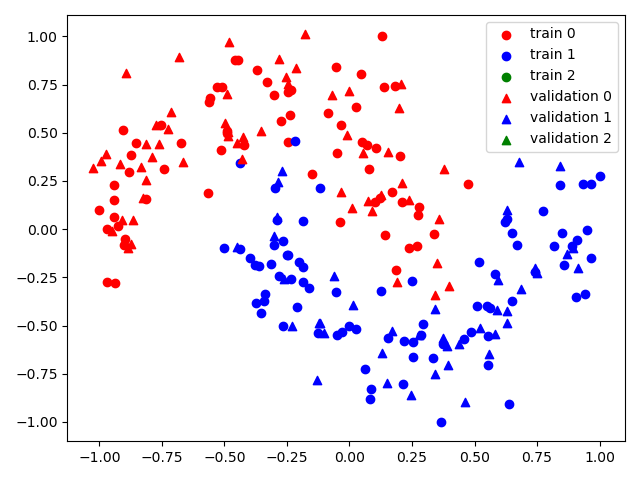
\includegraphics[width=\thisfigurewidth\textwidth]{figures/fig_dataset_moons.png} \\
      (a) & (b) & (c) \\[6.5pt]
      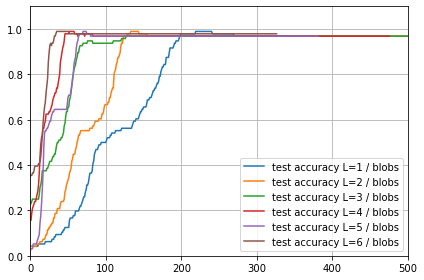
\includegraphics[width=\thisfigurewidth\textwidth]{figures/test_acc_blobs_lr=0_1.png} & 
      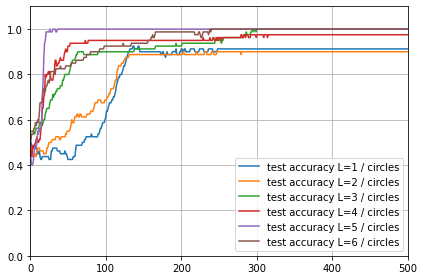
\includegraphics[width=\thisfigurewidth\textwidth]{figures/test_acc_circles_lr=0_1.png} &
      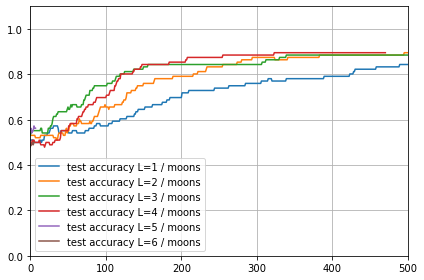
\includegraphics[width=\thisfigurewidth\textwidth]{figures/test_acc_moons_lr=0_001.png} \\
      (d) & (e) & (f) \\[6.5pt]
      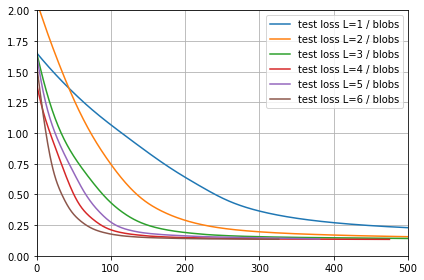
\includegraphics[width=\thisfigurewidth\textwidth]{figures/test_loss_blobs_lr=0_001.png} & 
      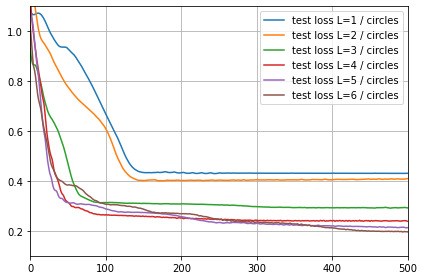
\includegraphics[width=\thisfigurewidth\textwidth]{figures/test_loss_circles_lr=0_1.png} &
      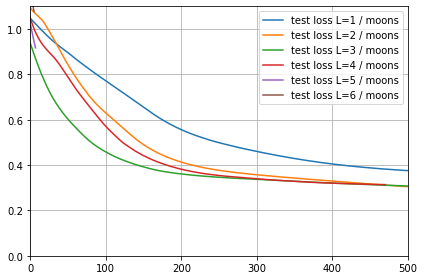
\includegraphics[width=\thisfigurewidth\textwidth]{figures/test_loss_moons_lr=0_001.png} \\
      (g) & (h) & (i) \\[6.5pt]
    \end{tabular}
    \caption{leiras}
    \label{fig:exactdiagonalization}
\end{figure}

\begin{figure}[H]
    \centering
    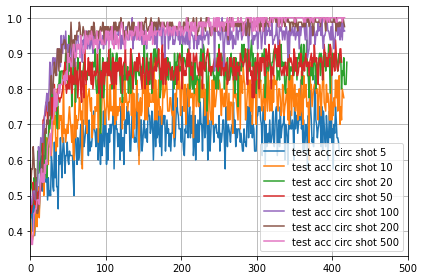
\includegraphics[width=0.5\textwidth]{figures/classifier-test-acc-shots.png}
    \caption{}
    \label{fig:single_layer_regression}
\end{figure}

\subsection{CV-VQE for the Bose-Hubbard model}
The Bose-Hubbard model introduced first by Gersch and Knollman in 1963 for the description of interacting spinless bosons on a lattice, such as ultracold bosonic atoms on an optical lattice
\cite{BoseHubbardOriginal,ColdAtomtHubbard}. This model has also gained popularity because it is found to be an adequate model for the description of the Superfluidity-Mott insulator (SF-MI) transition, which has been experimentally demonstrated \cite{SuperfluidityMottTransition,Greiner2002}.
We chose this model, because an exact diagonalization of the Bose-Hubbard Hamiltonian with respect to a finite dimensional Fock-basis is possible and thus the model is numerically solvable. This enables the verification of the correctness of the results given by our variational quantum solver for small problem instances.
\par
The Bose Hubbard model which we used in our simulations is defined by the following Hamiltonian expressed with the bosonic creation and annihillation operators:
\begin{equation}
     H = -t\sum\limits_{i=1}^{M-1}( a_{i}^\dagger  a_{i+1} +  a_{i+1}^\dagger  a_{i}) + \frac{U}{2}\sum\limits_{i=1}^{M} n_i^2 ,
     \label{eq:bhhamiltonian}
\end{equation}
where $M$ is the number of bosonic modes in the system. If we restrict the total number of bosons in the system to be $N$, the dimension of the restricted Fock-space is
\begin{equation}
    D = \frac{(N+M-1)!}{N!(M-1)!},
\end{equation}
which explosively grows with the system size. Therefore finding the groundstate of the Bose-Hubbard Hamiltonian for larger systems can be intractable even on classical supercomputers, making quantum computers, especially continuous-variable quantum computers a potential candidate for solving these problems in the future.
Compared to the original definition of the Bose-Hubbard Hamiltonian, we omitted the term $-\mu\sum\limits_{i}^{M} n_i$, because it is not relevant in our particular experiments.

\subsubsection{Solving the model by exact diagonalization}
\nd{Analytic solution by diagonalization}
If we want to calculate the groundstate of a Bose-Hubbard model, then we need to solve the 
eigenvalue-problem of Hamiltonian \ref{eq:bhhamiltonian}.
Of course a general Fock-space corresponding to a bosonic system is infinite-dimensional, therefore
we have to restrict the system so that a maximum of $N$ particles are allowed in each mode:
\begin{align*}
|0,0, ..., 0\rangle, |0,0, ..., N\rangle, |0,0, ..., 1, N\rangle, ... |N,N,...,N\rangle.
\end{align*}
Then, we can relabel the Fock-states so that each Fock basis has its own unique label $j$:
\begin{equation}
|n_{M-1}, n_{M-2}, ... n_{1}, n_{0}\rangle = \left|\sum\limits_{k=0}^{M-1}n_{k}(N+1)^{k}\right\rangle.
\end{equation}
This is useful, because with these relabeled states we can calculate the matrix elements of the new 
Hamiltonian:
\begin{equation}
    H_{jj'} = \bra{j}H\ket{j'} = \langle n_{M-1}, n_{M-2}, ... n_{1}, n_{0}| H |n'_{M-1}, n'_{M-2}, ... n'_{1}, n'_{0}\rangle
\end{equation}
We can further reduce the dimension of the Hilbert space if we prescribe that the total number of photons
must be $N$:
\begin{equation*}
    \sum\limits_kn_k = N.
\end{equation*}
In this case for example if the number of modes is $M=4$ and the total number of particles is $N=4$,
the dimension of the restricted Hilbert-space is only $35$.

The resulting matrix $H_{jj'}$ is usually a sparse matrix (see fig. \ref{fig:exactdiagonalization}),
and can be diagonalized using existing software.
\begin{figure}[H]
    \centering
    \begin{tabular}{cc}
      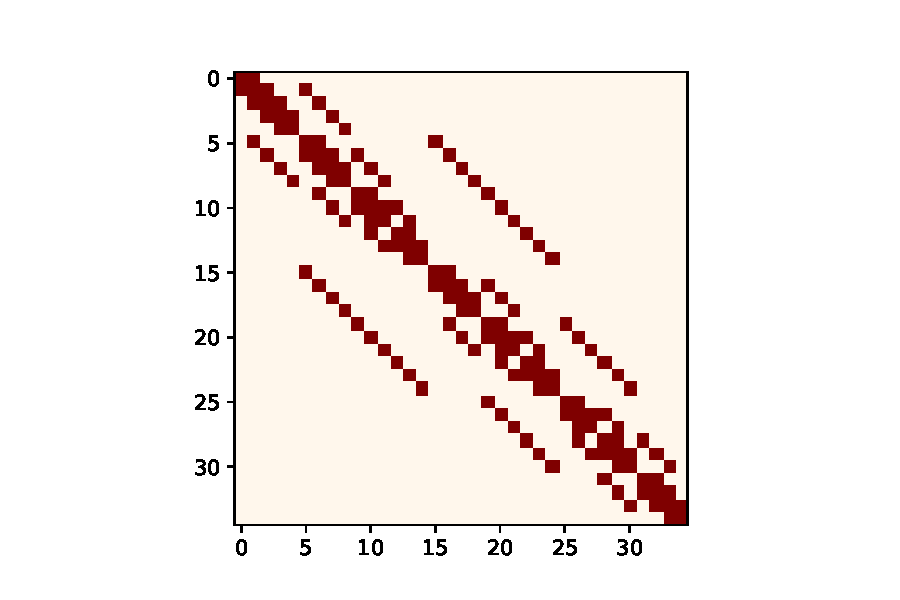
\includegraphics[height=0.2\textheight]{figures/real_fock_matrix_M=4_cutoff=4_t=-0_5_U=-0_5.pdf} & 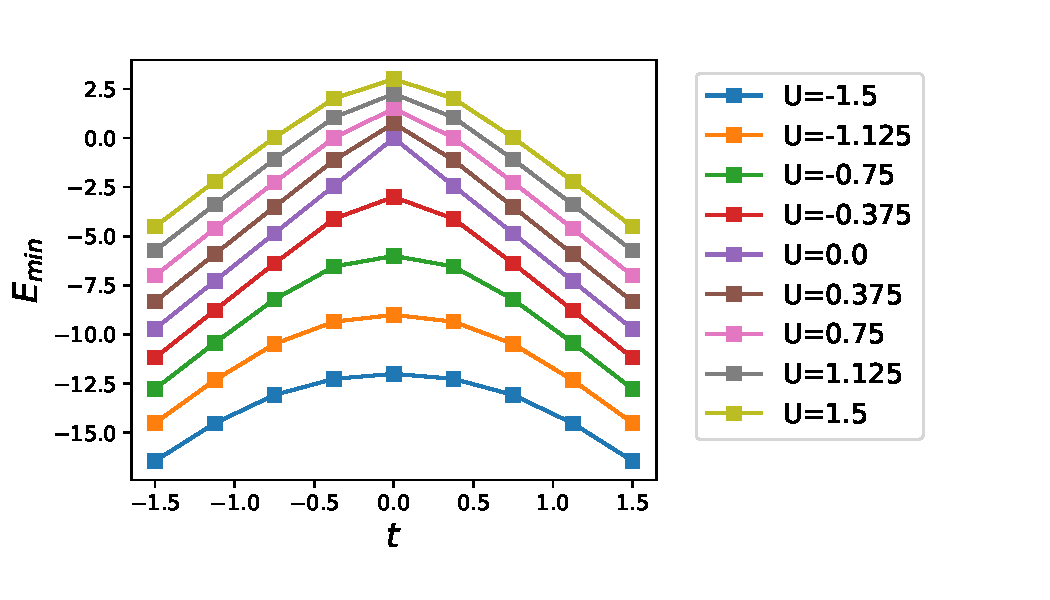
\includegraphics[height=0.2\textheight]{figures/diagonalized_solutions_M=4_cutoff=4.pdf} \\
      (a) & (b) \\[6pt]
    \end{tabular}
    \caption{(a) Visual representation of a sparse Hamiltonian matrix $H_{jj'}$ for a Bose-Hubbard model
    with $\dim(\mathcal H)=35$.
    Darker points show the non-zero elements in the matrix (b) Numerical solutions of the ground-state
    energy for different $U$ and $t$ values.}
    \label{fig:exactdiagonalization}
\end{figure}

\subsubsection{Variational solutions}
VQEs introduced in section \ref{sec:vqe} are shown to be effective for simulating
different fermionic quantum systems, like molecules or metals 
\cite{Wei2020-QCHEM, VQE-HARTREE-FOCK, Kandala2017-VQE-QCHEM, PhysRevX-VQE-QCHEM}.
In this chapter we demonstrate a photonic VQE for finding the ground-state energy of a Bose-Hubbard model.
Furthermore, we show that stochastic gradient descent methods can be applied to the VQE to reduce
the number of shots required, and thus reduce the overall cost of finding the ground state energy
on a quantum hardware.
\par
The variational circuit $U(\pmb\theta)$ can be realized with sequences of quantum gates, in our case
photonic quantum gates.
Since we want the total number of particles in the system to be preserved during the simulations,
we must use photon-number preserving gates only. We composed each quantum layer from 
Beamsplitters, Kerr-gates and Cross-Kerr-gates (see fig. \ref{fig:single_layer_vqe}).
\begin{figure}[H]
    \centering
    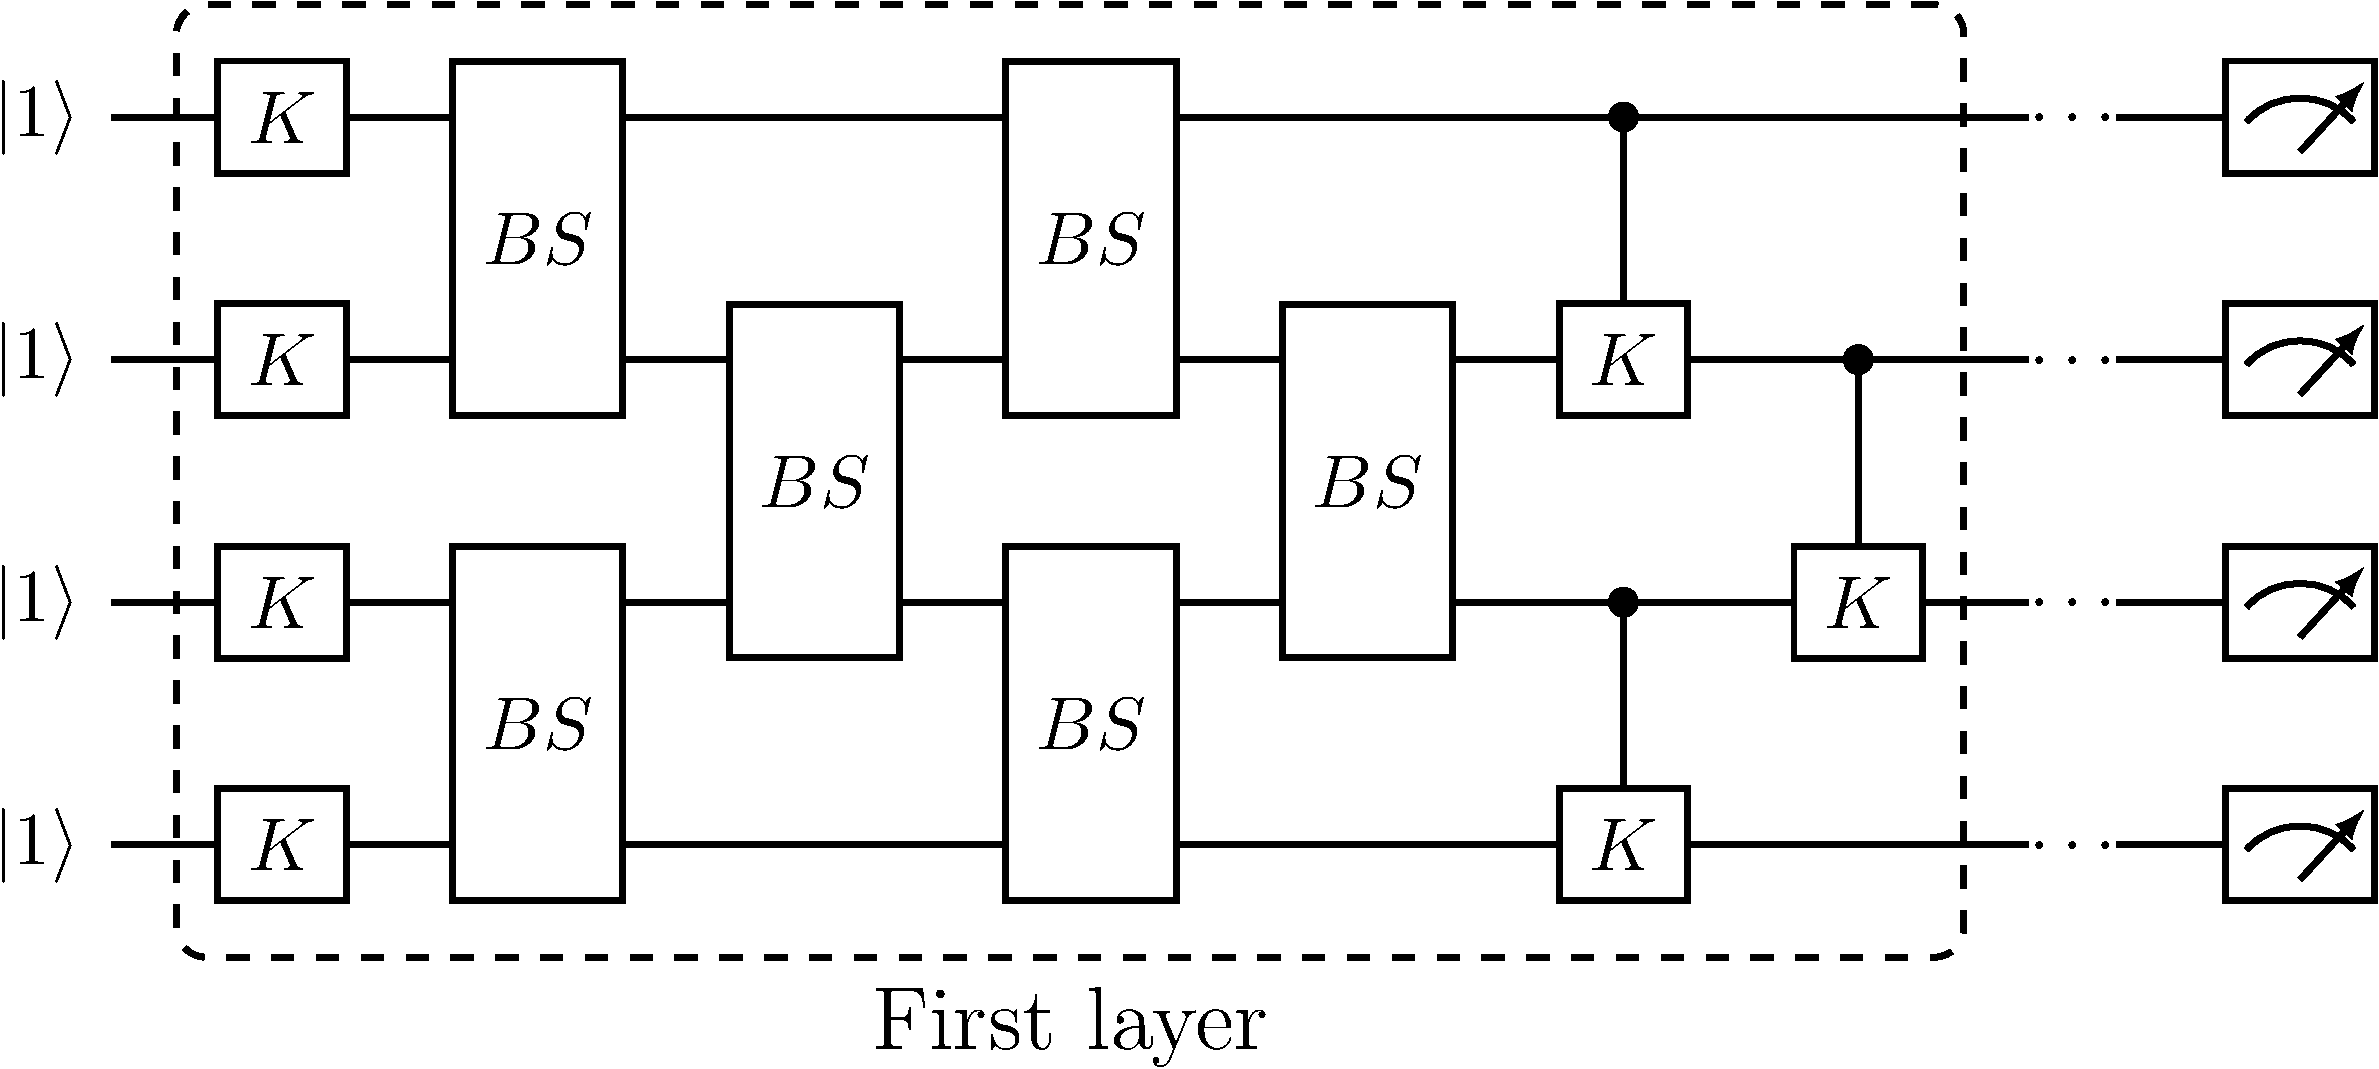
\includegraphics[width=0.66\textwidth]{figures/BH-Ansatz.pdf}
    \caption{Illustration of a variational ansatz circuit with its first layer. Initially, each of the four qumodes contain a
    single photon. The layer is built up from Kerr-gates, CrossKerr gates and Beamsplitters, which are passive optical gates, so the
    total number of photons is preserved.}
    \label{fig:single_layer_vqe}
\end{figure}
Throughout the numerical experiments, we set initially one single photon in each of the four qumodes i.e.
$\ket{\psi_0}=\ket{1}^{\otimes M}$, and applied a number of identical quantum layers 
followed by quadrature measurements.
\begin{figure}[H]
    \centering
    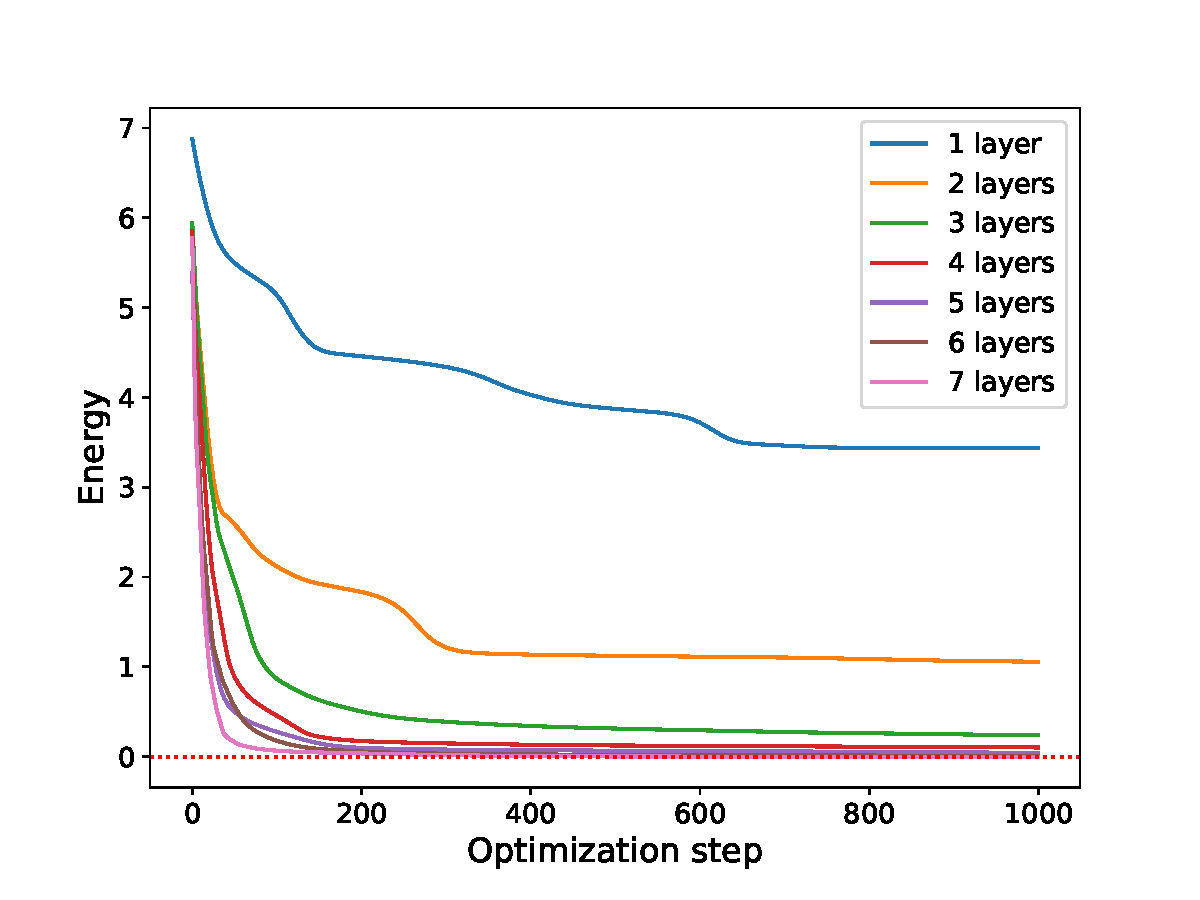
\includegraphics[width=0.66\textwidth]{figures/BH-layersearch-2.pdf}
    \caption{}
    \label{fig:single_layer_vqe}
\end{figure}

\begin{figure}[H]
    \centering
    \begin{tabular}{cc}
      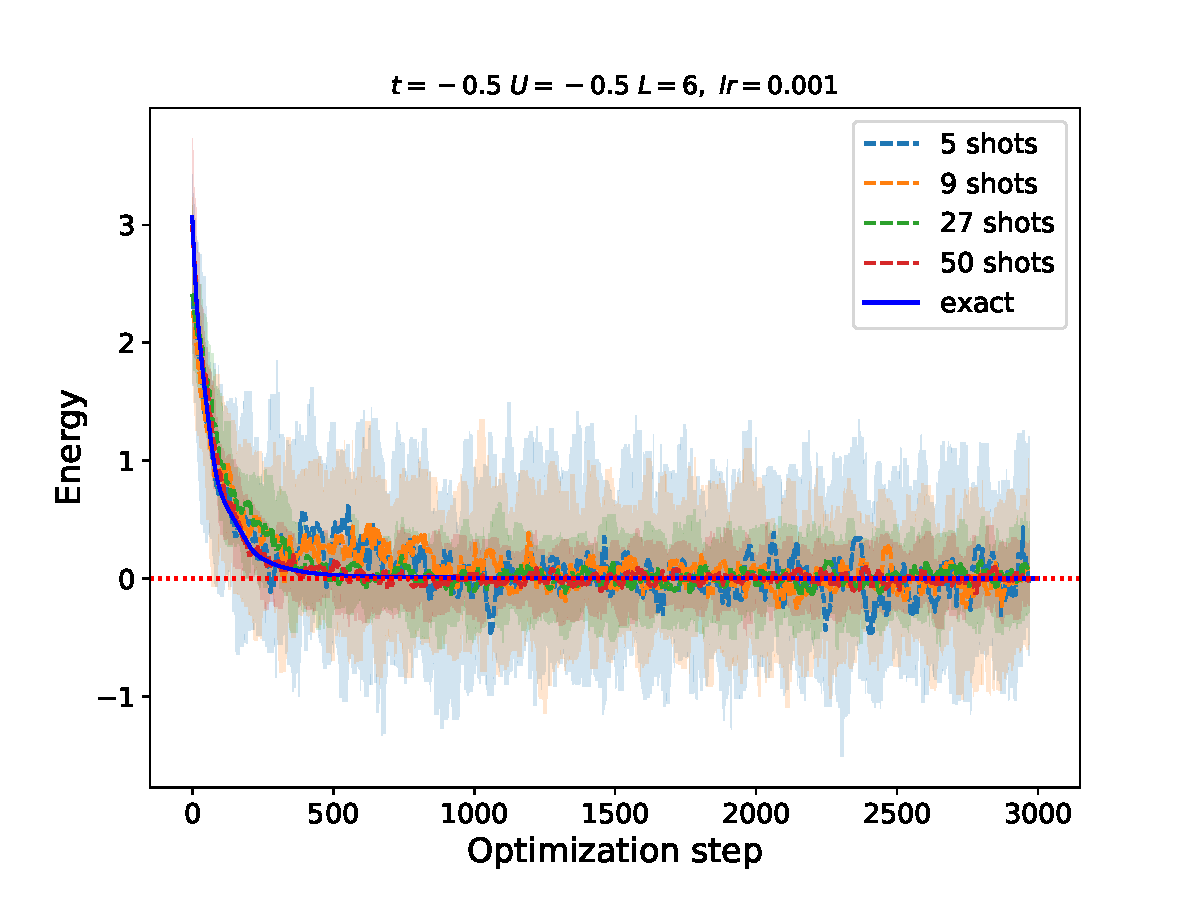
\includegraphics[width=0.5\textwidth]{figures/BH-stoch-L=6-t=-0_5-U=-0_5-lr=0_001-shots=5-50.pdf} &   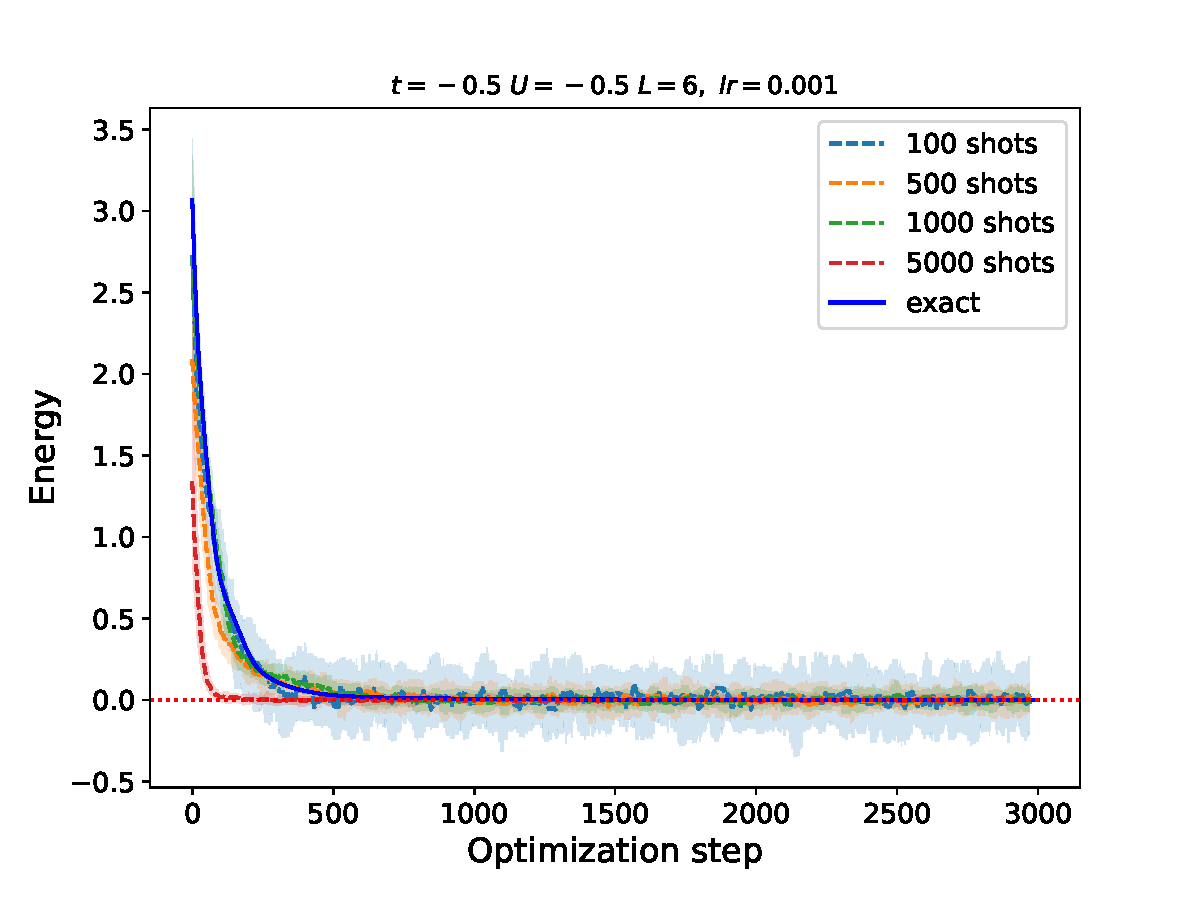
\includegraphics[width=0.5\textwidth]{figures/BH-stoch-L=6-t=-0_5-U=-0_5-lr=0_001-shots=100-5000.pdf} \\
    (a) first & (b) second \\[6pt]
     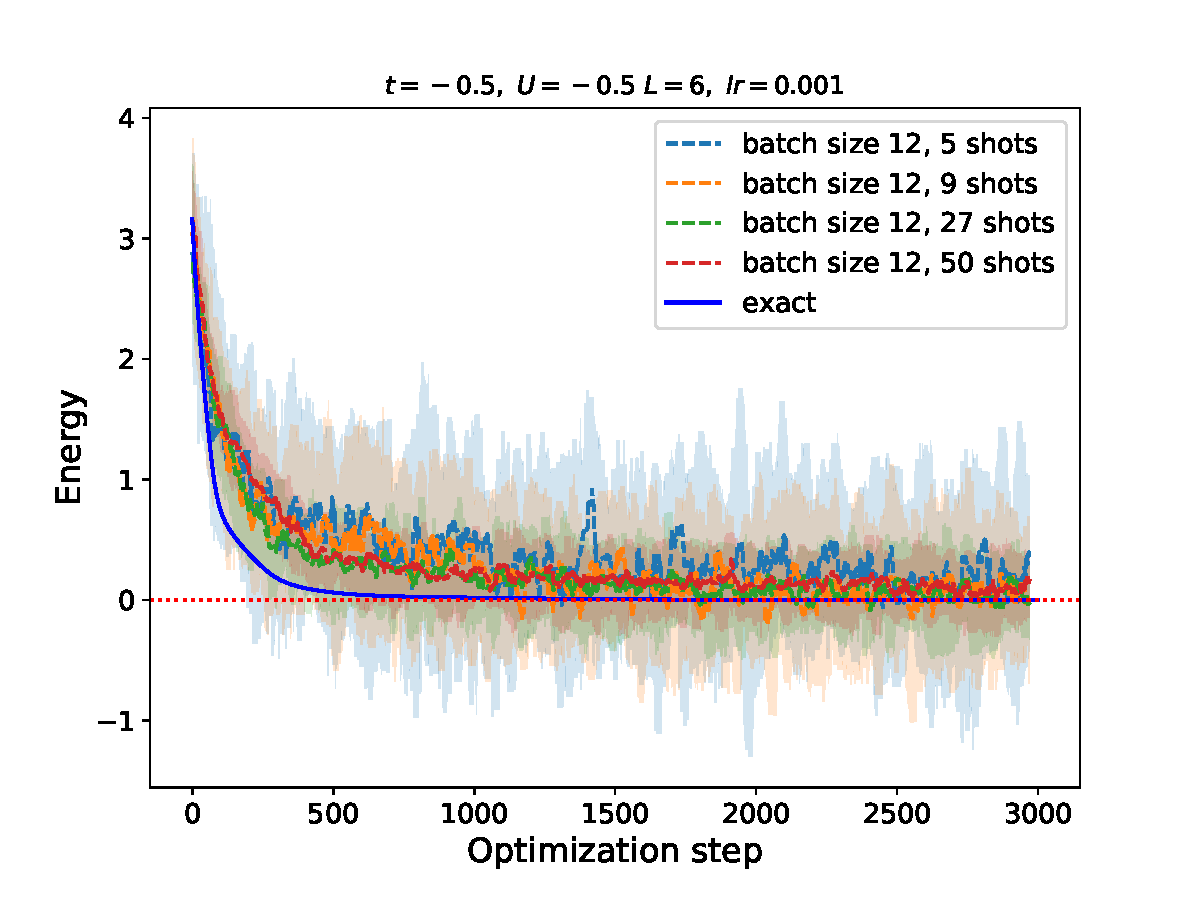
\includegraphics[width=0.5\textwidth]{figures/BH-doublystoch-bs=12-L=6-t=-0_5-U=-0_5-lr=0_001-shots=5-50.pdf} &   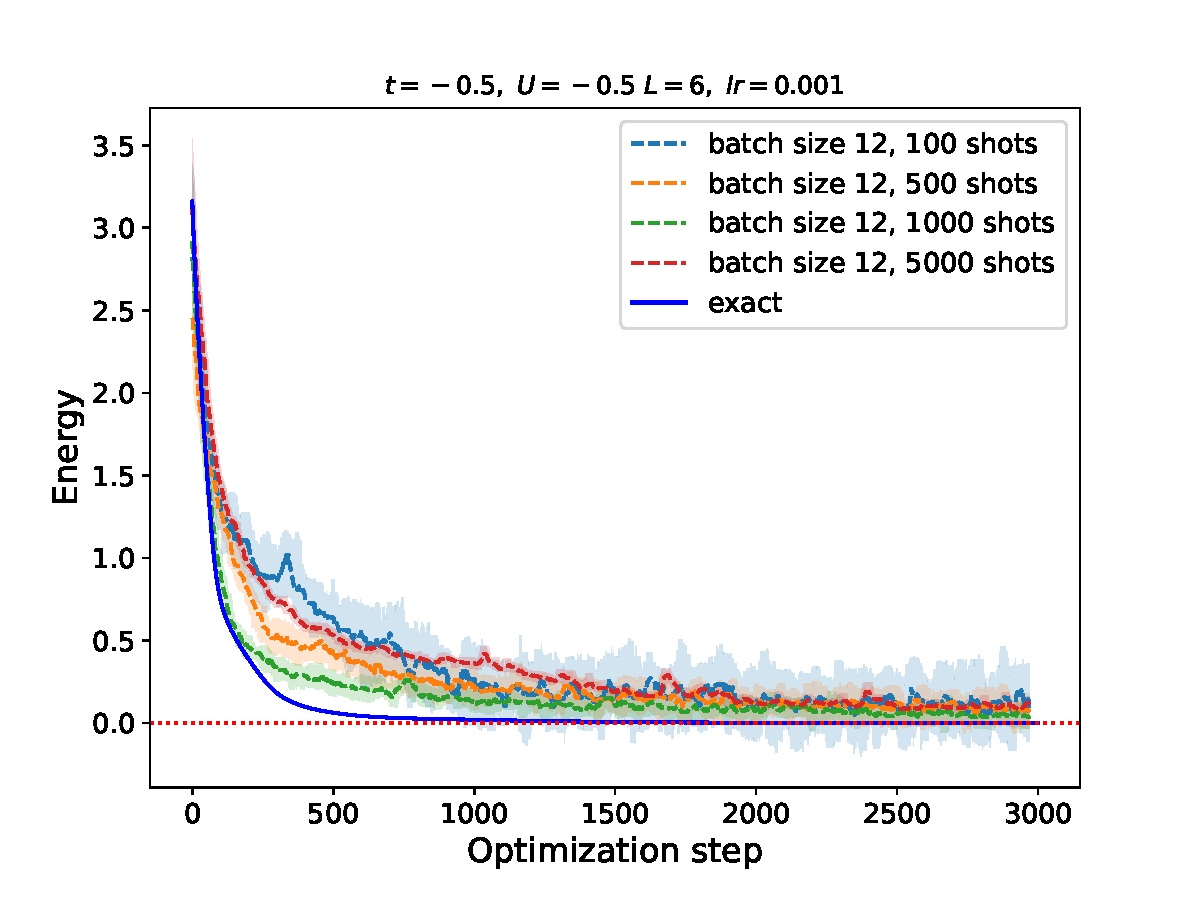
\includegraphics[width=0.5\textwidth]{figures/BH-doublystoch-bs=12-L=6-t=-0_5-U=-0_5-lr=0_001-shots=100-5000.pdf} \\
    (c) third & (d) fourth \\[6pt]
    \end{tabular}
    \caption{caption}
\end{figure}

\bibliography{references}
%%%%%%%%%%%%%%%%%%%%%%%%%%%%%%%%%%%%%%%%%%%%%%%%%%%%%%%%%%%%%%%%%%%%%%%%%%%%%%%%%%%%%%%%%%%%%%%%%%%
%%%%%%%%%%%%%%%%%%%%%%%%%%%%%%%%%%%%%%%%%%%%%%%%%%%%%%%%%%%%%%%%%%%%%%%%%%%%%%%%%%%%%%%%%%%%%%%%%%%
%
%                    APPENDIX
%
%%%%%%%%%%%%%%%%%%%%%%%%%%%%%%%%%%%%%%%%%%%%%%%%%%%%%%%%%%%%%%%%%%%%%%%%%%%%%%%%%%%%%%%%%%%%%%%%%%%
%%%%%%%%%%%%%%%%%%%%%%%%%%%%%%%%%%%%%%%%%%%%%%%%%%%%%%%%%%%%%%%%%%%%%%%%%%%%%%%%%%%%%%%%%%%%%%%%%%%


\appendix
\section{Coherent states}
\label{appendix:coherent}
A coherent state is the eigenstate of $\hat a$:
\begin{equation*}
    \hat a \ket{\alpha} = \alpha\ket{\alpha}
\end{equation*}
\begin{align*}
    \ket\alpha = \sum\limits_{n=0}^{\infty}\ket n\braket{n|\alpha}
\end{align*}
we have
\begin{align*}
    &\hat a\ket\alpha = \alpha\ket\alpha \implies \braket{n|\hat a|\alpha}=\alpha\braket{n|\alpha}
\end{align*}
and 
\begin{align*}
    &\hat a^{\dagger}\ket n = \sqrt{n+1}\ket{n+1} \implies \bra n \hat a = \sqrt{n+1}\bra{n+1}\\
    &\implies \braket{n|\hat a|\alpha} = \sqrt{n+1}\braket{n+1|\alpha} = \alpha\braket{n|\alpha}\\
    &\implies \braket{n|\alpha} = \frac{\alpha}{\sqrt n}\braket{n-1|\alpha} = \dots = \frac{\alpha^n}{\sqrt{n!}}
    \braket{0|\alpha}
\end{align*}
therefore,
\begin{align*}
    \ket\alpha = \sum\limits_{n=0}^{\infty}\frac{\alpha^n}{\sqrt{n!}}\braket{0|\alpha}\ket n
\end{align*},
The value of $\braket{0|\alpha}$ can be calculated from the normalization condition
$\braket{\alpha|\alpha}\overset{!}{=}1$. Since
\begin{align*}
    &\ket\alpha = \braket{0|\alpha}\sum\limits_{n=0}^{\infty}\frac{\alpha^n}{\sqrt{n!}}\ket n \\ 
    &\bra\alpha = \braket{\alpha|0}\sum\limits_{k=0}^{\infty}\frac{(\alpha^*)^k}{\sqrt{k!}}\bra k,
\end{align*}
we have 
\begin{align*}
    1\overset{!}{=} \braket{\alpha|\alpha} & = 
    \left(\braket{\alpha|0}\sum\limits_{k=0}^{\infty}\frac{(\alpha^*)^k}{\sqrt{k!}}\bra k\right)
    \left(\braket{0|\alpha}\sum\limits_{n=0}^{\infty}\frac{\alpha^n}{\sqrt{n!}}\ket n\right)\\
    &=\braket{\alpha|0}\braket{0|\alpha}\sum\limits_{k=0}^{\infty} \sum\limits_{n=0}^{\infty}
    \frac{(\alpha^*)^k\alpha^n}{\sqrt{k!n!}}\braket{k|n} \\
    &=\braket{\alpha|0}\braket{0|\alpha}\sum\limits_{k=0}^{\infty} \sum\limits_{n=0}^{\infty}
    \frac{(\alpha^*)^k\alpha^n}{\sqrt{k!n!}}\delta_{kn}\\
    &= |\braket{0|\alpha}|^2 \sum\limits_{n=0}^{\infty} \frac{(|\alpha|^2)^n}{n!} = |\braket{0|\alpha}|^2e^{|\alpha|^2}.
\end{align*}
\begin{equation*}
    \implies \braket{0|\alpha} = e^{i\varphi}e^{-\frac{|\alpha|^2}{2}}
\end{equation*}
And so, a coherent state can be written as 
\begin{equation*}
    \ket\alpha = e^{i\varphi}e^{\frac{-|\alpha|^2}{2}}\sum\limits_{n=0}^{\infty}\frac{\alpha^n}{\sqrt{n!}}\ket n
\end{equation*}
\section{Mathematical preliminaries}

\subsection{Hilbert spaces}
\begin{definition}
    \textbf{Hilbert-space}\\
    Given a field $T$ (real or complex), a vector space $\mathcal H$ endowed with an inner product, is called a Hilbert-space, if
    it is a complete metric space with respect to the distance function induced by the inner product.
    \\
    The inner product is a map $\braket{\cdot|\cdot}:\mathcal{H}\times\mathcal{H} \rightarrow T$, 
    for which $\forall x,y,z \in \mathcal H$:
    \begin{itemize}
        \item $\braket{x|x} \geq 0$
        \item $\braket{x|x} = 0 \Longleftrightarrow x = \bb 0 \in \mathcal H$
        \item $\braket{x|y} = \braket{y|x}^*$, where $^*$ denotes complex conjugation.
        \item $\braket{x|\alpha y + \beta z} = \alpha\braket{x|y} + \beta\braket{x|z}$, where $\alpha, \beta \in T$
    \end{itemize}
    The norm induced by this inner product is a map $||\cdot||:\mathcal H \rightarrow T$ defined as
    \begin{equation*}
        ||x||=\sqrt{\braket{x|x}},
    \end{equation*}
    And the metric induced by this norm is defined as
    \begin{equation*}
        d(x,y) = ||x - y|| = \sqrt{\braket{x - y|x - y}}.
    \end{equation*}
    The space $\mathcal H$ is said to be complete if every Cauchy-sequence is convergent with respect to the norm, and
    the limit is in $\mathcal H$. That is, each sequence ${x_1, x_2, ... }$, for which 
    \begin{equation*}
        \forall \varepsilon > 0 ~ \exists N(\varepsilon) ~\textrm{so, that}~ n>m>N(\varepsilon) \implies ||x_n - x_m||<\varepsilon.
    \end{equation*}
\end{definition} 

\begin{definition}
    \textbf{Linear functional}\\
    Let $\mathcal H$ be a Hilbert-space over the field $T$. Then, the map $\varphi:\mathcal H \rightarrow T$ is  
    called a linear functional, if
    \begin{equation*}
        \varphi(\alpha x + \beta y) = \alpha \varphi(x) + \beta \varphi(y),~
        \forall \alpha, \beta \in T,\, x, y \in \mathcal H.
    \end{equation*}
\end{definition}

\begin{definition}
    \textbf{Dual space}\\
    Given a Hilbert-space $\mathcal H$, its dual space, $\mathcal H^*$ is the space of all continuous linear
    functionals from the space H into the base field.
    The norm of an element in $\mathcal H^*$ is 
    \begin{equation*}
        ||\varphi||_{\mathcal H^*} \overset{def}{=} \underset{||x||=1,\, x \in \mathcal H}{\sup} |\varphi(x)|.
    \end{equation*}
\end{definition}

\begin{theorem}
    \textbf{Riesz representation theorem}\\
    For every element $y \in \mathcal H$, there exists a unique element $\varphi_{y} \in \mathcal H^*$, defined by
    \begin{equation*}
        \varphi_{y}(x) = \braket{y| x},~\forall x \in \mathcal H.
    \end{equation*}
    The mapping $y \mapsto \varphi_{y}$ is an antilinear mapping i.e. $\alpha y_1 + \beta y_2 
    \mapsto \alpha^* \varphi_{y_1} + \beta^* \varphi_{y_2}$, and the Riesz-representation theorem states 
    that this mapping is an antilinear isomorphism. The inner product in $\mathcal H^*$ satisfies 
    \begin{equation*}
        \braket{\varphi_{x}|\varphi_{y}} = \braket{x|y}^* = \braket{y | x}.
    \end{equation*}
    Moreover, $||y||_{\mathcal H} = ||\varphi_{y}||_{\mathcal H^*}$.
\end{theorem}

\begin{definition}
    \textbf{Dirac-notation}\\
    From now on, the elements in $\mathcal H$ will be denoted by $\ket x$ and their corresponding
    element in $\mathcal H^*$ as $\bra x$.
\end{definition}

\subsection{Linear operators on Hilbert spaces}

\begin{definition}
    \textbf{Linear operators}\\
    A map $\hat A: \mathcal H_1 \rightarrow \mathcal H_2$ is a linear operator, if 
    \begin{equation*}
        \hat A (\alpha\ket x + \beta\ket y) = \alpha (\hat A \ket x) + \beta (\hat A \ket y).
    \end{equation*}
\end{definition}

\begin{remark}
    If not stated otherwise, we will assume that $\mathcal H_1 = \mathcal H_2 = \mathcal H$.
\end{remark}

\begin{remark}
    Operators will be denoted with a hat ($\hat{\cdot}$).
\end{remark}

\begin{definition}
    \textbf{Bounded linear operators}\\
    A linear operator $\hat A: \mathcal H \rightarrow \mathcal H$ is bounded, if 
    \begin{equation*}
        \exists m \in \mathbb R : |\braket{v|\hat A | v}| \leq m\braket{v|v},\, \forall \ket v \in \mathcal H
    \end{equation*}
\end{definition}

\begin{remark}
    The set of all bounded operators on $\mathcal H$ is denoted $\mathcal{B(H)}$.
\end{remark}


\begin{definition}
    \textbf{Commutators and anticommutators}\\
    Since operators usually do not commute, its useful to define their commutator and anticommutator:
    \begin{align*}
        &[\hat A, \hat B] = \hat A\hat B - \hat B\hat A\\
        &\{\hat A, \hat B\} = \hat A\hat B + \hat B\hat A
    \end{align*}
\end{definition}

\begin{definition}
    \textbf{Operator norm}\\
    The operator norm of an operator $\hat A$ is defined as 
    \begin{equation*}
        ||\hat A|| \overset{def}{=} \inf\{c\geq 0 : ||\hat A\ket v || \leq c ||\ket v||,\,\forall \ket v \in \mathcal H \}
    \end{equation*}
\end{definition}

\begin{definition}
   \textbf{Trace-class operators}\\
   An operator $\hat A$ is called trace-class if it admits a well defined and finite trace 
   $\Tr{\hat A} = \sum\limits_j\braket{j|\hat A|j}$
\end{definition}

\begin{definition}
    \textbf{Positive operators}\\
    An operator $\hat A$ is called positive if $\braket{v|\hat A|v} \geq 0,\,\forall \ket v \in \mathcal{H}$.
    If $\hat A = \sum\limits_j \lambda_j \ket j \bra j$ then $\hat A$ is positive if $\lambda_j \geq 0$.
\end{definition}

\begin{definition}
    \textbf{Projections}
    An operator $\Pi:\mathcal H \rightarrow \mathcal H$ is a projection if $\Pi^2=\Pi$.
\end{definition}

\subsection{Hermitian Operators, Unitary Operators, Spectral theorem, Hadamard-lemma}
\begin{definition}
    \textbf{Hermitian adjoint}
    \\Consider a \textbf{bounded} linear operator $\hat A: \mathcal H \rightarrow \mathcal H$. The hermitian adjoint of 
    $\hat A$ is a bounded linear operator $\hat A^\dagger : \mathcal H \rightarrow \mathcal H$ which satisfies
    \begin{equation}
        \bra y \hat A \ket x = \left( \bra x \hat A^\dagger \ket y \right)^*, ~\forall \ket x, \ket y \in \mathcal H.
    \end{equation}
\end{definition}

\begin{definition}
    \textbf{Hermitian operators}
    \\ A bounded linear operator $\hat H : \mathcal H\rightarrow \mathcal H$ is Hermitian if 
    \begin{equation}
        \hat H = \hat H^\dagger, \textrm{ i.e. } \hat H\ket x = \hat H^\dagger \ket x, ~\forall \ket x \in \mathcal H.
    \end{equation}
\end{definition}

\begin{definition}
    \textbf{Unitary operator}
    \\A bounded linear operator $\hat U : \mathcal H\rightarrow \mathcal H$ is unitary if 
    \begin{equation}
        \hat U\hat U^\dagger = \hat U^\dagger \hat U = 1, \textrm{ in other words, } \hat U^{\dagger} = \hat U^{-1}. 
    \end{equation}
\end{definition}

\begin{definition}
    \textbf{Eigenvalues and eigenvectors}
    \\Consider bounded linear operator $\hat A$. If exist a vectors $\ket k \in \mathcal H$ such that
    \begin{equation}
        \hat A \ket k = \lambda_k\ket k,
    \end{equation}
    then $\ket k$ is called an eigenvector of $\hat A$ and $\lambda k$ is the corresponding eigenvalue.
\end{definition}

An important property of Hermitian operators is that they can be diagonalized with real eigenvalues. 
This is formally stated by the spectral theorem:
\begin{theorem}
    \textbf{The Spectral theorem}
    \\Let $\hat A$ be a bounded Hermitian operator on some Hilbert-space $\mathcal H$. Then there exists an orthonormal
    basis in $\mathcal H$ which consists of the eigenvectors of $\hat A$ and each eigenvalue of $\hat A$ is real.
\end{theorem}
This means that any bounded Hermitian operator $\hat H$ can be decomposed as 
\begin{equation}
    \hat H = \sum\limits_{k}\lambda_k \hat P_k = \sum\limits_{k}\lambda_k \ketbra{k}{k}
\end{equation}
where $\lambda_k$ and $\ket k$ are the eigenvalues and eigenvectors of $\hat H$.


\begin{definition}
    \textbf{Exponential of operators}
    If $X$ is a linear operator, we can define the exponential of $X$:
    \begin{equation*}
        e^X = \sum\limits_{n=0}^\infty \frac{X^n}{n!} 
    \end{equation*}
\end{definition}
\textbf{Important}:
The product of exponentials of operators generally isn't equal to the exponential of their sum:
\begin{equation*}
    e^{X}e^{Y} = e^{Z(X,Y)}\neq e^{X+Y},
\end{equation*}
where $Z(X,Y)$ is given by the Baker-Campbell-Hausdorff formula:
\begin{align*}
    Z(X,Y) &= X + Y + \frac{1}{2}[X,Y] + \frac{1}{12}[X,[X,Y]] - \frac{1}{12}[Y,[X,Y]] -\frac{1}{24}[Y,[X,[X,Y]]] \\
    & - \frac{1}{720}([[[[X,Y],Y],Y],Y] + [[[Y,X],X],X],X]) + ...
\end{align*}
It is however equal if $[X,Y]=0$:
\begin{equation*}
    \textrm{if}\,[X,Y]=0 \implies  e^{X}e^{Y} = e^{X+Y}
\end{equation*}
There are 2 important special cases:
\begin{theorem}
    \textbf{The Hadamard-lemma}
    \begin{equation*}
        e^XYe^{-X} = Y + [X,Y] + \frac{1}{2!}[X,[X,Y]] + \frac{1}{3!}[X,[X,[X,Y]]] + ...
    \end{equation*}
\end{theorem}

\begin{theorem}
    If $X$ and $Y$ commute with their commutator, i.e. $[X, [X,Y]] = [Y, [X,Y]] = 0$, then:
    \begin{equation*}
        e^Xe^Y = e^{X+Y+\frac{1}{2}[X,Y]}
    \end{equation*}
\end{theorem}

\begin{theorem}
    If $[X,Y] = sY$ with $s\in\mathbb{C}, s\neq 2i\pi n, n\in \mathbb Z$ then:
    \begin{equation*}
        e^Xe^Y = \exp\left(X + \frac{s}{1-e^{-s}}Y \right)
    \end{equation*}
\end{theorem}

\subsection{Pure and mixed quantum states}
\begin{definition}
    \textbf{Quantum states}\\
    A quantum state of a quantum system is a mathematical entity that provides a probability distribution 
    for the outcomes of each possible measurement on the system.
\end{definition}

\begin{definition}
    \textbf{Pure quantum states}\\
    Pure quantum states are quantum states that can be described by a vector $\ket\psi$ of norm 1. 
\end{definition}
If one multiplies a pure quantum state by a complex scalar $e^{i\alpha}$, then the new state is 
physically equivalent to the former, thus $\ket\psi$ and $e^{i\alpha}\ket\psi$ are 
the same pure state.
The transformation $\ket\psi\rightarrow e^{i\alpha}\ket\psi$ does not change the outcomes of measurements on the state,
however the phase $\alpha$ is important in quantum algorithms.
\begin{example*}
    For example, the states $\frac{1}{\sqrt 2}(\ket 0 + e^{i\pi}\ket 1)$ and $\frac{1}{\sqrt 2}(\ket 0 + e^{i\frac{\pi}{2}}\ket 1)$
    are not the same quantum state, but in both states there is 50-50 percent probability of measuring $\ket 0$ and $\ket 1$.
\end{example*}

\begin{definition}
    \textbf{Density Matrix}\\
    A quantum state $\hat\rho$ is a trace-1, self-adjoint, positive semidefinite operator.
    The set of quantum states is
    \begin{equation*}
        \mathcal{S(H)} = \{ \hat\rho : \hat\rho \geq 0, \hat\rho=\hat\rho^{\dagger}, \Tr{\hat\rho} = 1 \}
    \end{equation*}
    A quantum state is pure if and only if $\hat\rho^2=\hat\rho$. 
    Also, if $\rho$ is a pure state, then it can be written as $\hat\rho = \ketbra{\psi}{\psi}$.
    The operator $\rho$ is called the \textit{density operator} or \textit{density matrix}.
    \label{def:densityop}
\end{definition}


\end{document}